\documentclass{article}
\usepackage[utf8]{inputenc}
\usepackage[margin=0.5in,includefoot]{geometry}
\usepackage[export]{adjustbox}

% Header and Footer Setup
\usepackage{fancyhdr}
\pagestyle{fancy}
\fancyhead{}
\fancyfoot{}
\fancyfoot[R]{\thepage}
\renewcommand{\headrulewidth}{0pt}
\renewcommand{\footrulewidth}{0pt}
%
%Graphics Setup
\usepackage{graphicx}
\usepackage{float}
\usepackage{subfig}


%list setup
\usepackage{amssymb}
\renewcommand{\labelitemi}{$\blacktriangleright$}
\renewcommand{\labelitemii}{$\bullet$}
\renewcommand{\labelitemiii}{$\circ$}

%Source Code setup
\usepackage{xcolor}
\usepackage{listings}

\definecolor{mGreen}{rgb}{0,0.6,0}
\definecolor{mGray}{rgb}{0.5,0.5,0.5}
\definecolor{mPurple}{rgb}{0.58,0,0.82}
\definecolor{backgroundColour}{rgb}{0.95,0.95,0.92}

\lstdefinestyle{CStyle}{
    backgroundcolor=\color{backgroundColour},   
    commentstyle=\color{mGreen},
    keywordstyle=\color{magenta},
    numberstyle=\tiny\color{mGray},
    stringstyle=\color{mPurple},
    basicstyle=\footnotesize,
    breakatwhitespace=false,         
    breaklines=true,                 
    captionpos=b,                    
    keepspaces=true,                 
    numbers=left,                    
    numbersep=5pt,                  
    showspaces=false,                
    showstringspaces=false,
    showtabs=false,                  
    tabsize=2,
    language=C
}
%


\begin{document}

\begin{titlepage}

	\begin{flushright}
	\textsc{\large May 9, 2021} \\
	\end{flushright}
	\begin{center}
	\Large{\bfseries GTU Department of Computer Engineering \\ CSE344 - Spring 2021 \\ Homework 4 Report  } \\
	\end{center}
	\topskip0pt
	\vspace*{\fill}
	\begin{center}
	\Large{\bfseries Akif Kartal \\ 171044098 }
	\end{center}
	\vspace*{\fill}

\end{titlepage}

\cleardoublepage
\section{Problem Definition}
The problem is to implement \textbf{producer-consumer} problem by using POSIX threads and Semaphores as initiation to POSIX threads. 

\section{Solution}
The homework was finished as expected in homework pdf file. 
\subsection{Some Problems and Solutions}
\subsubsection{Semaphore Usage}
In order to provide synchronization between threads I used \textbf{6 POSIX unnamed semaphore} common between threads.
Followings are my semaphores;
\begin{lstlisting}[style=CStyle]
    sem_init(&run, 0, 0);
    sem_init(&mutex, 0, 1);
    sem_init(&empty, 0, 10);
    sem_init(&full, 0, 0);
    sem_init(&busy, 0, 0);
    sem_init(&dataMutex, 0, 1);
\end{lstlisting}
Usage purpose of each semaphore will be explained in detail coming pages.
\subsubsection{Thread Creation}
\subsubsection*{Main Thread}
Main thread is main function of program and it is responsible to initialize important variables such as queue, semaphores, money etc. Also reading queue.
\subsubsection*{Thread G}
This thread is detached thread so its different than other. Also it is filling the queue therefore we need to \textbf{pass as parameter} the queue
to the this thread. Note that queue is \textbf{not} global, it is in main thread. See the code;
\begin{lstlisting}[style=CStyle]
 pthread_attr_t attr;
 pthread_attr_init(&attr);
 pthread_attr_setdetachstate(&attr, PTHREAD_CREATE_DETACHED);

 /*create G thread*/
 queue *stdQueue = createQueue();
 pthread_create(&idG, &attr, threadG, (void *)stdQueue);
 pthread_attr_destroy(&attr);
\end{lstlisting}
\subsubsection*{Threads of student-for-hire}
Here, we have threads as many as number of student but important thing is \textbf{they will use same thread function}. Therefore, 
we need to design a communication mechanism between each student thread and main thread. My solution is following;
\subsubsection*{Setting Up the Student Threads}
Since, these threads are using same function somehow we need to distinguish each other. In order to do that we will pass an encapsulated data,
which contains information about student for each thread while creating. Note that after creating \textbf{they need to wait} until all of them
initialized with it's data. See the code;
\cleardoublepage
\begin{lstlisting}[style=CStyle]
 //data for each student to pass to the it's thread
 typedef struct info
 {
    char name[41];
    double price;
    double speed;
    double quality;
    double income;
    int solvedCount;
    int index;
    int isBusy;
    int isNotified;
    sem_t *notify;
    sem_t *startSolve;
    char currentHw;
    pthread_t id;
 } student;
\end{lstlisting}
In this data, semaphores will be used to communicate and synchronize. Other variables are clear.
\subsubsection*{Creating Students}
\begin{lstlisting}[style=CStyle]
 //N = number of student(itu,ytu etc.)
 pthread_t tids[N];
 student hiredStds[N];
  
 /*create hired students threads and init them*/
 for (int i = 0; i < N; i++)
 {
    pthread_create(&tids[i], NULL, threadStd, &hiredStds[i]);
 }
 initStudents(hiredStds, fdStd, N, tids);
 mainPrintStudents(hiredStds,N);
 /*post that students can run now*/
 if (sem_post(&run) == -1)
        errExit("sem_post");
 /*student thread*/
 void *threadStd(void *info)
 {
    if (safeSemWait(&run) == -1)
        pthread_exit(NULL);
    if (sem_post(&run) == -1)
        errExit("sem_post");
    if (exitSignal)
        pthread_exit(NULL);
    student *this = (student *)info;
    ...
 }
       
\end{lstlisting}

\subsubsection{Communication and Synchronization Problems}
\subsubsection*{Main Thread and Thread G}
I this two thread we have \textbf{producer-consumer} problem. In order to solve this problem I used 3 semaphore 
which are \textbf{full, empty, mutex}. \\ \\
Solution;
\cleardoublepage
\textbf{Producer(Thread G)}
\begin{lstlisting}[style=CStyle]
	do
    {
        nextHw = readOneChar(fdHw);
        if (nextHw != 'x' && !isFinished)
        {
            if (safeSemWait(&empty) == -1)
                pthread_exit(NULL);
            if (exitSignal)
                pthread_exit(NULL);
            if (safeSemWait(&mutex) == -1)
                pthread_exit(NULL);
            if (isFinished)//money run out
                break;

            gNewHwMsg(nextHw,money);
            addRear(p, nextHw);

            if (sem_post(&mutex) == -1)
                errExit("sem_post");
            if (sem_post(&full) == -1)
                errExit("sem_post");
        }
    } while (nextHw != 'x' && !isFinished);
\end{lstlisting}
\textbf{Consumer(Main Thread)}
\begin{lstlisting}[style=CStyle]
	while (money > 0 && !isFinished)
	{
        if (safeSemWait(&full) == -1)
            cleanAndExit(hiredStds,tids,N,stdQueue);
        if (exitSignal)
            cleanAndExit(hiredStds,tids,N,stdQueue);
        if (safeSemWait(&mutex) == -1)
            cleanAndExit(hiredStds,tids,N,stdQueue);
        if (!isQueueEmpty(stdQueue)){
            index = findStudent(hiredStds, getFront(stdQueue));
            if (hiredStds[index].price <= money)
            {
                if (safeSemWait(&dataMutex) == -1)
                    cleanAndExit(hiredStds,tids,N,stdQueue);
                    
                //remove hwk and update values  
                hiredStds[index].currentHw = removeFront(stdQueue);
                hiredStds[index].isNotified += 1;
                money = money - hiredStds[index].price;
                hiredStds[index].income += hiredStds[index].price;
                hiredStds[index].solvedCount += 1;
                
                //notify the selected student to start solving it
                if (sem_post(hiredStds[index].notify) == -1)
                    errExit("sem_post");
                if (sem_post(&dataMutex) == -1)
                    errExit("sem_post");
                    
                //wait first student to start
                if (safeSemWait(hiredStds[index].startSolve) == -1)
                    cleanAndExit(hiredStds,tids,N,stdQueue);
								if (sem_post(&mutex) == -1)
									errExit("sem_post");
								if (sem_post(&empty) == -1)
									errExit("sem_post");
            }
            else{
            	break;
        	}
        else{
            break;
        }
	}
\end{lstlisting}
In this code piece some semaphores belongs to main thread and hired student communication and synchronization.
Also, I determine Queue data structure \textbf{upper-bound limit is 10}.
\subsubsection*{Main Thread and Hired Students}
I this two thread we have \textbf{communication and synchronization} problems. In order to solve this problems I used 3 semaphores 
which are \textbf{run, busy, dataMutex}. Also in info data, for each student we are using \textbf{notify and startSolve} seamphores. \\ \\
Usage;
\begin{itemize}
	\item \textbf{run}: When a student thread created, it will wait to initialize its data by main thread.
	\item \textbf{busy}: When all students are busy main thread will wait until one student post to busy thread.
	\item \textbf{dataMutex}: Both students and main thread are updating student info, therefore in order to avoid race
	condition we will use this semaphore.
	\item \textbf{notify}: notify a student when it was chosen.
	\item \textbf{startSolve}: After notification was send wait the student to start \textbf{not} completely finished solving.
\end{itemize}
The solution of these problems is following;\\ \\
\textbf{Main Thread}
\begin{lstlisting}[style=CStyle]
	index = findStudent(hiredStds, getFront(stdQueue));
	if (index == -1)
	{
		//all of them are busy
		int counter;
		if (sem_getvalue(&busy, &counter) == -1)
			errExit("sem_get");
		if (counter > 0){
			if (safeSemWait(&busy) == -1)
            	cleanAndExit(hiredStds,tids,N,stdQueue);
		}
		if (safeSemWait(&busy) == -1)
        	cleanAndExit(hiredStds,tids,N,stdQueue);
		index = findStudent(hiredStds, getFront(stdQueue));
	}
	if (hiredStds[index].price <= money)
	{
		if (safeSemWait(&dataMutex) == -1)
        	cleanAndExit(hiredStds,tids,N,stdQueue);
			
		//remove hwk and update values  
		hiredStds[index].currentHw = removeFront(stdQueue);
		hiredStds[index].isNotified += 1;
		money = money - hiredStds[index].price;
		hiredStds[index].income += hiredStds[index].price;
		hiredStds[index].solvedCount += 1;
		
		//notify the selected student to start solving it
		if (sem_post(hiredStds[index].notify) == -1)
			errExit("sem_post");
		if (sem_post(&dataMutex) == -1)
			errExit("sem_post");
			
		//wait first student to start
		 if (safeSemWait(hiredStds[index].startSolve) == -1)
         	cleanAndExit(hiredStds,tids,N,stdQueue);
	}
	if (exitSignal)
    	cleanAndExit(hiredStds,tids,N,stdQueue);
\end{lstlisting}
\cleardoublepage
\textbf{Hired Student}
\begin{lstlisting}[style=CStyle]
while (!isFinished || this->isNotified)
{
	stdWaitMsg(this->name);
	//wait notificition
	if (safeSemWait(this->notify) == -1)
    	pthread_exit(NULL);
		
	if (this->isNotified){
	
		if (safeSemWait(&dataMutex) == -1)
        	pthread_exit(NULL);
        	
		this->isBusy = 1;
		stdSolvingMsg(this->name,this->price,money,this->currentHw);
		
		//release start mutex
		if (sem_post(this->startSolve) == -1)
			errExit("sem_post");
		if (sem_post(&dataMutex) == -1)
			errExit("sem_post");

		//simulate solving
		sleep(6 - (int)this->speed);

		 if (safeSemWait(&dataMutex) == -1)
         	pthread_exit(NULL);
			
		this->isNotified -= 1;
		this->isBusy = 0;

		if (sem_post(&dataMutex) == -1)
			errExit("sem_post");
		int counter;
		if (sem_getvalue(&busy, &counter) == -1)
			errExit("sem_get");
		if (counter == 0){
			if (sem_post(&busy) == -1)
				errExit("sem_post");
		}
	}
	else
		break;
}
\end{lstlisting}
\subsubsection{CTRL-C Handling}
In order to terminate on CTRL-C interrupt, I used \textbf{sigaction} function from \textbf{signal.h} library. But in order to do that we need to wait
each thread return and then give resources back. Also, while in sem\_wait(), we need to do this anyway threfore I wrote \textbf{my safeSemWait() function.}
See my solution; \\ \\
\textbf{Handler and Usage}
\cleardoublepage

\begin{lstlisting}[style=CStyle]
    //handler function
	volatile __sig_atomic_t exitSignal = 0;
	void exitHandler(int signal)
	{
    	if (signal == SIGINT)
    	{
        	exitSignal = 1;
    	}
	}
    //my sem_wait
	int safeSemWait(sem_t *sem){
    	if (sem_wait(sem) == -1){
        	if (errno == EINTR && exitSignal == 1){
           		return -1;
        	} else{
            	errExit("sem_wait interrupt");
        	}
    	}
    	return 0;
	}
	//usage in main thread
	if (exitSignal)
     	cleanAndExit(hiredStds,tids,N,stdQueue);
    //or
    if (safeSemWait(&full) == -1)
       cleanAndExit(hiredStds,tids,N,stdQueue);
       
    //usage in other threads
    if (exitSignal)
    	pthread_exit(NULL);
    //or
    if (safeSemWait(&dataMutex) == -1)
    	pthread_exit(NULL);
    
\end{lstlisting}
\textbf{Cleaner function after an exit signal}
\begin{lstlisting}[style=CStyle]
    //cleaner function
void cleanAndExit(student stds[],pthread_t ids[],int n,queue *head){
    printf("Termination signal received, closing.\n");
    if (sem_post(&dataMutex) == -1)
        errExit("sem_post");
    if (sem_post(&mutex) == -1)
        errExit("sem_post");
    if (sem_post(&empty) == -1)
        errExit("sem_post");
    for (int i = 0; i < n; ++i) {
        if (sem_post(stds[i].notify) == -1)
            errExit("sem_post");
    }
    for (int i = 0; i < n; i++)
    {
        if (!pthread_equal(pthread_self(), ids[i]))
            pthread_join(ids[i], NULL);
    }
    freeQueue(head);
    sem_destroy(&run);
    sem_destroy(&mutex);
    sem_destroy(&full);
    sem_destroy(&dataMutex);
    sem_destroy(&busy);
    sem_destroy(&empty);
    destroy(stds,n);
    exit(EXIT_SUCCESS);
}
    
\end{lstlisting}
\section{References that was used} 
\begin{itemize}
	\item Advanced Linux Programming Book Chapter 4 Threads.
	\item Week-8 slides synchronization: Bounded buffer case in producer consumer problem.
\end{itemize}
\cleardoublepage
\section{Test Result}
I tried to obey output example in homework pdf. In following output all decisions belongs to CPU. \\
A simple test result is following; \\
\begin{figure}[H]
    \centering
    \subfloat[\centering Homework File]{{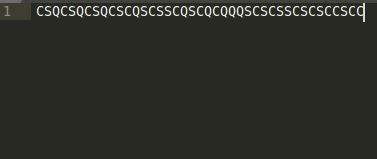
\includegraphics[width=5cm]{res4.JPG} }}%
    \qquad
    \subfloat[\centering Hired Students]{{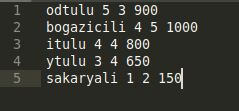
\includegraphics[width=5cm]{res3.JPG} }}%
    \caption{Files Before Test}
    \label{fig:example}
\end{figure}
\begin{figure}[H]
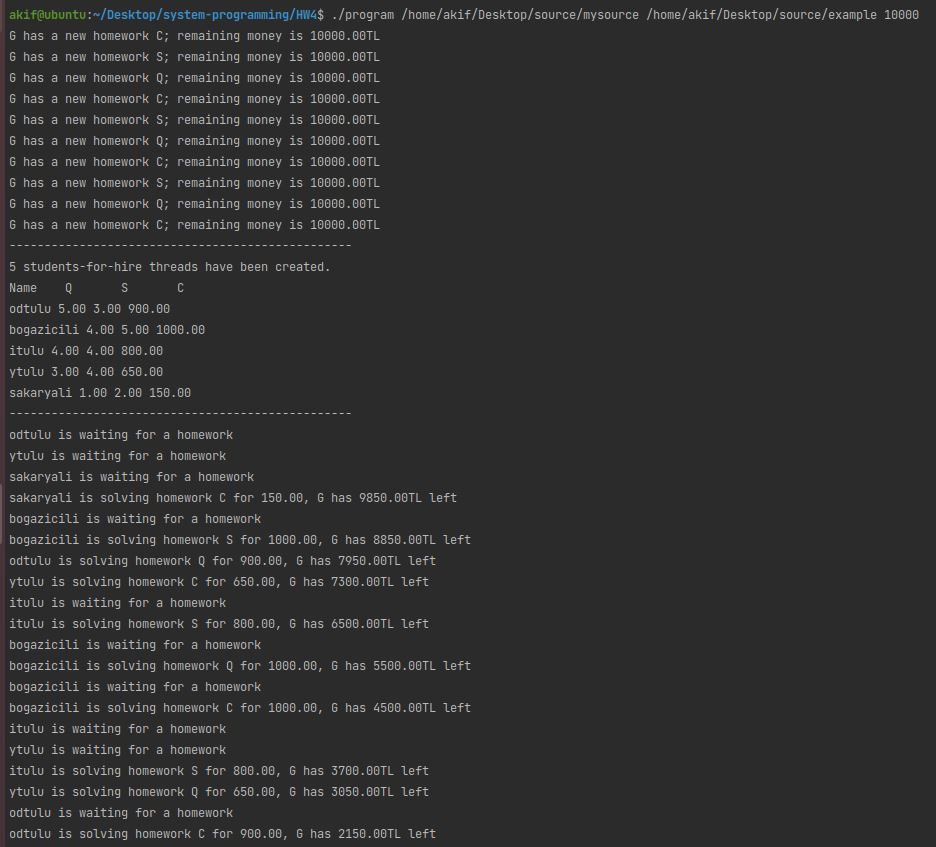
\includegraphics[width=1\textwidth, left]{res1.JPG}		
\end{figure}                              
\cleardoublepage
\begin{figure}[H]
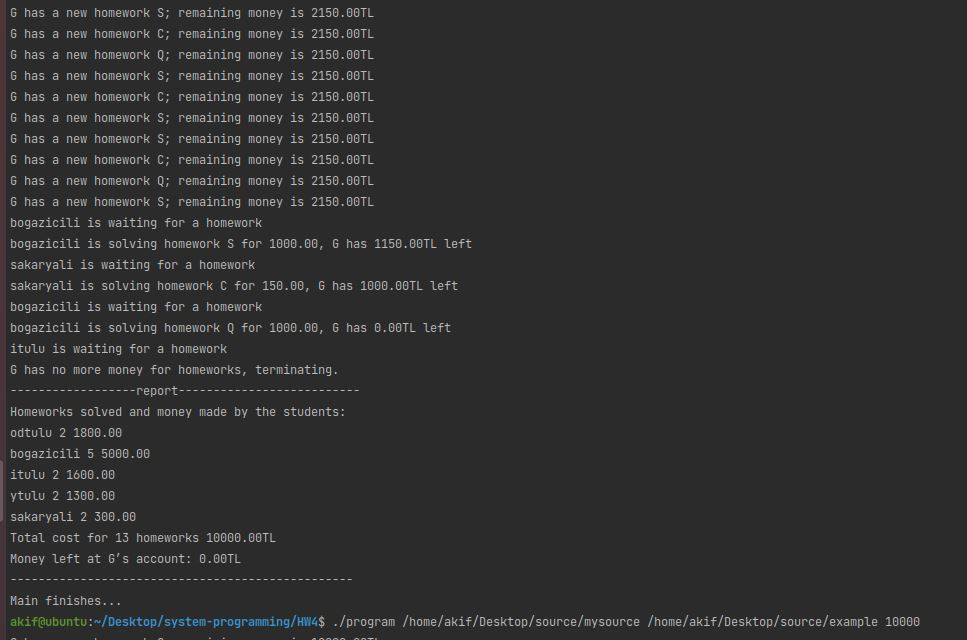
\includegraphics[width=1\textwidth, left]{res2.JPG}
\caption[Optional caption]{}
\label{}		
\end{figure}    
\end{document}